\chapter{Basic Concepts}

A task can be seen as a sequence of actions and a deadline must be associated to each one of them.\\
We, therefore, are after is a definition of a formal model that identifies what these tasks or actions are and associate deadlines with them.

\section{Real-Time Tasks}
\definition{Real-Time Task ($\tau_i$)}{stream of jobs (or instances) $J_{i,k}$, or, in other terms, a sequence of activities that is activated periodically or aperiodically}

Each job $J_{i,k} =  (r_{i,k}, c_{i,k}, d_{i,k})$ is characterised by the following quantities:
\begin{itemize}
    \item{\makebox[1cm]{$r_{i,k}$\hfill}activation time}\pside{activation time}\\
    It is the time at which a task becomes ready for execution; it is also referred as \textit{request time} or \textit{release time}. 
    \item{\makebox[1cm]{$c_{i,k}$\hfill}computation time}\pside{computation time}\\
    Time necessary to the processor for executing the job without interruption.
    \item{\makebox[1cm]{$d_{i,k}$\hfill}absolute deadline}\pside{absolute deadline}\\
    time before which a job should be completed to avoid damage to the system.
    \item{\makebox[1cm]{$f_{i,k}$\hfill}finishing time}\pside{finishing time}\\
    The time at which a job finishes its execution
    \item{\makebox[1cm]{$\rho_{i,k}$\hfill}response time}\pside{response time}\\
    The time at which a job finishes its execution. Formally this quantity is the difference between the finishing time and the activation time.
    \[\rho_{i,k}  = f_{i,k} - r_{i,k}\]
\end{itemize}
Furthermore, since each task $i$ is a sequence of jobs, we need to differentiate between them. That is why each job $J_{i,k}$ is uniquely identified by its task index $i$ and the $k$-th activation of the $i$-th task.\\
In addition, we will say that job $J_{i,k}$ respects its deadline if $f_{i,k} \le d_{i,k}$.



\begin{figure}[!ht]
    \centering
    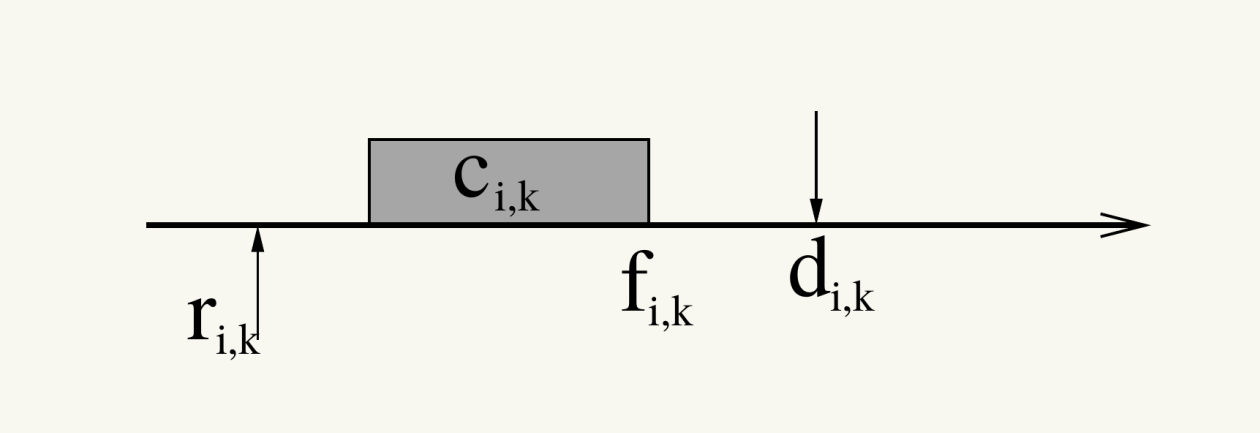
\includegraphics[width = 0.8\textwidth]{images/image01.png}
    \caption{Graphical representation of Mathematical model of a Task}
    \label{fig:image01}
\end{figure}

This mathematical definition of a job in a real-time task holds regardless of the nature of the task itself. In fact, we can identify three different types of tasks: Periodic tasks, Aperiodic Tasks and Sporadic Tasks.
Each of them holds different properties and a different mathematical representation.

\subsection{Periodic Tasks}

\definition{Periodic Task}{A periodic task $\tau_i = (C_i, D_i, T_i)$ is a stream of jobs $J_{i,k}$, with:
\begin{align*}
r_{i,k+1} &= r_{i,k} + T_i\\
d_{i,k} &= r_{i,k} + D_i\\
C_i &= \max_k\{c_{i,k}\}
\end{align*}
}
where:
\begin{itemize}
    \item{\makebox[1cm]{$T_i$\hfill}\textbf{Period}}\pside{Period}
    \item{\makebox[1cm]{$D_i$\hfill}\textbf{Relative Deadline}}\pside{Relative Deadline}
    \item{\makebox[1cm]{$C_i$\hfill}\textbf{Worst-Case Execution Time (WCET)}}\pside{Worst-Case Execution Time (WCET)}
    \item{\makebox[1cm]{$R_i$\hfill}\textbf{Worst-Case Response Time (WCRT)}}\pside{Worst-Case Response Time (WCRT)}
    \[R_i = \max_k \{\rho_{i,k}\}=\max_k \{f_{i,k} - r_{i,k}\}\]
\end{itemize}
For the task to be correctly scheduled, it must be $R_i \le D_i$

A periodic task has a regular structure (called \side{cycle}), in the sense that:
\begin{itemize}
\item it is activated periodically with a period of $T_i$
\item it executes a computation
\item when the computation terminates, it suspends waiting for the next period
\end{itemize}

Hence, its fundamental implementation can be represented as:
\begin{lstlisting}[language=C++]
void *PeriodicTask(void *arg)
{
	<initialization>;
	<start periodic timer, period = T>;
	while (condition)
	{
		<read sensors>;
		<update outputs>;
		<update state variables>;
		<wait next activation>;
	}
}
\end{lstlisting}

\subsection{Aperiodic Tasks}

\definition{Aperiodic Task}{Aperiodic tasks are not characterised by periodic arrivals, meaning that:
\begin{itemize}
    \item A minimum interarrival time between activations does not exist
    \item Sometimes, aperiodic tasks do not have a particular structure
\end{itemize}
}

Aperiodic tasks can model tasks responding to events that occur rarely (e.g. a mode change) or tasks responding to events with irregular structure (e.g. bursts of packets from the network,\dots).

\subsection{Sporadic Tasks}
Sporadic tasks are aperiodic tasks characterised by a \textbf{Minimum Interarrival Time (MIT)} between jobs.
In this sense they are similar to periodi tasks, but while a periodic task is activated by a periodic timer, a sporadic task is activated by an external event. (e.g. the arrival of a packet from the network)

Hence, its fundamental implementation can be represented as:
\begin{lstlisting}[language=C++]
    void *SporadicTask(void *arg)
    {
        <initialization>;
        while (condition)
        {
            <computation>;
            <wait events>;
        }
    }
\end{lstlisting}
Formally: 
\definition{Sporadic Task}{A sporadic task $\tau_i = (C_i, D_i, T_i)$ is a stream of jobs $J_{i,k}$, with:
\begin{align*}
    r_{i,k+1} &\ge r_{i,k} + T_i\\
    d_{i,k+1} &= r_{i,k} + D_i\\
    C_i &= \max_k\{c_{i,k}\}
\end{align*}
}
where:
\begin{itemize}
    \item{\makebox[1cm]{$T_i$\hfill}\textbf{Minimum Interarrival Time (MIT)}}\pside{Minimum Interarrival Time (MIT)}
    \item{\makebox[1cm]{$D_i$\hfill}\textbf{Relative Deadline}}\pside{Relative Deadline}
    \item{\makebox[1cm]{$C_i$\hfill}\textbf{Worst-Case Execution Time (WCET)}}\pside{Worst-Case Execution Time (WCET)}
    \item{\makebox[1cm]{$R_i$\hfill}\textbf{Worst-Case Response Time (WCRT)}}\pside{Worst-Case Response Time (WCRT)}
    \[R_i = \max_k \{\rho_{i,k}\}=\max_k \{f_{i,k} - r_{i,k}\}\]
\end{itemize}
For the task to be correctly scheduled, it must be $R_i \le D_i$.

\section{Task Criticality}
% types of task constraints
A deadline is said to be \textit{hard} if a deadline miss causes a critical failure in the system, whereas a task is said to be a \side{hard real-time task} if all its deadlines are hard, which means that all the deadlines must be guaranteed before starting the task, i.e.
\[\forall j, \rho_{i,j} \le D_i \qquad\Rightarrow\qquad R_i \le D_i\]



\example{Hard Real-Time Task}{The controller of a mobile robot, must detect obstacles and react within a time dependent on the robot speed, otherwise the robot will crash into the obstacles}

A deadline is said to be \textit{soft} if a deadlien miss causes a degradation in the \side{Quality of Service (QoS)}, but is not a catastrophic event, whereas a task is said to be a \side{soft real-time task} if it has soft deadlines.\\
In other terms, some deadlines can be missed without compromising the correctess of the system, but the number of missed deadlines must be kept under control, because the \textit{quality} of the results depend on the number of missed deadlines.

Unline the hard real-time task, soft real-time tasks can be difficult to characterize, particularly:
\begin{itemize}
\item What's the tradeoff between \textit{non compromising the system correctness} and \textit{not considering missed deadlines}?
\item Moreover, some way to express the QoS experienced by a soft real-time task is needed
\end{itemize}

Examples of QoS definitions could be
\begin{itemize}
\item no more than X consecutive deadlines can be missed
\item no more that X deadlines in an interval of time $T$ can be missed
\item the \side{deadline miss probability} must be less than a specified value, i.e.
\[P\{f_{i,j} > d_{i,j}\} \le R_{max}\]
\item the \side{deadline miss ratio} must be less than a specified value, i.e.
\[\cfrac{\text{number of missed deadlines}}{\text{total number of deadlines}} \le R_{max}\]
\item the maximum \side{tardiness} must be less than a specified value, i.e.
\[\cfrac{R_i}{D_i} < L\]
\item ...
\end{itemize}


\example{Audio and Video players}{Assuming a framerate of 25 fps, which imply a frame period of 40 ms, if a frame is played a little bit too late, the user might even be unable to notice any degration in the QoS, however, skipped frames can be disturbing.\\
In fact missing a lot of frames by 5 ms can be better than missing only a few frames by 40 ms.}
\example{Robotic Systems}{Some actuations can be delayed with little consequences on the control quality.}

In any case, soft real-time constraints does not mean no guarantee on dealines, given that tasks can have variable execution times between different jobs.\\
These execution times might depend on different factors:
\begin{itemize}
\item Input data
\item HW issues (cache effects, pipeline stalls, ...)
\item The internal state of the task
\item ...
\end{itemize}

\section{Schedulability analysis}
Schedulability analysis tries to answer the question: Given a task set $\mathcal{T}$, how can we guarantee if it is schedulable or not?
\subsection{Simulating the hyperperiod}
The first possibility is to simulate the system to check that no deadline is missed. The execution time of every job is set equal to the WCET of the corresponding task.\\

In the case of periodic tasks with no offsets it is sufficient to simulate the schedule until the \side{hyperperiod} (H = $lcm\{T_i\}$).\\
In the case of offsets $\phi_i = r_{i,0}$ it is sufficient to simulate until $2H + \phi_{max}$.\\
If tasks periods are prime numbers the hyperperiod can be very large!

In the case of sporadic tasks, we can assume them to arrive at the highest possible rate, so we fall back to the case of periodic tasks with no offsets.

\subsection{(Worst-Case) Response Time Analysis}
According to the methods proposed by Audsley et al., the longest response time $R_i$ of a periodic task $\tau_i$ is computed, at the critical instant, as the sum of its computation time and the interference $I_i$ of the higher priority tasks:
\[R_i = C_i + I_i\]
where:
\[I_i = \sum_{j=1}^{i-1} \ceil{\cfrac{R_i}{T_j}} C_j\]
Hence,
\begin{equation}
    \label{eq:equation0}
    R_i = C_i + \sum_{j=1}^{i-1} \ceil{\cfrac{R_i}{T_j}} C_j
\end{equation}

\definition{Critical instant}{The Critical instant for task $\tau_i$ occurs when job $J_{i,j}$ is released at the same time with a job in every high priority task}
It is straighforward to notice that if all the offsets of the task set are 0, the first job of every task is released at the \side{critical instant}.

A job $J_{i,j}$ released at the critical instant experiences the maximum response time for $\tau_i$:
\[\forall k,\quad \rho_{i,j}\ge\rho_{i,k}\]
No simple solution exists for this equation since $R_i$ appears on both sides of the equation. Thus, the worst-case response time of task $\tau_i$ is given by the smallest value of $R_i$ that satisfies equation \ref{eq:equation0}.
Notice, however, that only a subset of points in the interval $[0, D_i]$ need to be examined for feasibility. In fact, the interference on $\tau_i$ only increases when there is a release of a higher-priority task.

To simplify the notation, let $R_i^{(k)}$ be the $k$-th estimate of $R_i$ and let $I_i^{(k)}$ be the interference on task $\tau_i$ in the interval $[0, R_i^{(k)}]$
\begin{equation}
    I_i^{(k)} = \sum_{j=1}^{i-1} \ceil{\cfrac{R_i^{(k)}}{T_j}}C_j
    \label{eq:equation1}
\end{equation}
    Then the calculation of $R_i$ is performed as follows:
\begin{enumerate}
    \item Iteration starts with $R_i^{(0)} = \sum_{j=1}^{i} C_j$, which is the first point in time that $\tau_i$ could possibly complete
    \item The actual interference $I_i^k$ in the interval $[0, R_i^{(k)}]$ is computed by equation \ref{eq:equation1}
    \item If $I_i^{(k)} + C_i = R_i^{(k)}$, then $R_i^{(k)}$ is the actual worst-case response time of task $\tau_i$; that is, $R_i = R_i^{(k)}$. Otherwise, the next estimate is given by 
     \[R_i^{(k+1)} = I_i^{(k)} + C_i\]
     and the iteration continues from step 2. 
\end{enumerate}

Once $R_i$ is calculated, the feasibility of task $\tau_i$ is guaranteed if and only if $R_i \le D_i$.

The response time analysis is an efficient algorithm: in the worst case, the number of steps $N$ for the algorithm to converge is exponential and it depends on the total number of jobs of higher priority tasks in the interval $[0, D_i]$:
\[N \propto \sum_{h=1}^{i-1} \ceil{\cfrac{D_h}{T_h}}\]
If $s$ is the minimum granularity of the time, then in the worst case $N = \cfrac{D_i}{s}$. However, such worst case is very rare, usually the number of steps is low.

% can compute an exact result
% any priority assignment and preemptive scheduling

\subsection{Processor Demand Analysis}

Another necessary and sufficient test for checking the schedulability of fixed priority systems with constrained deadlines was proposed by Lehoczky, Sha and Ding. The test is based on the concept of Level-$i$ workload, defined as follows
\definition{Level-$i$ workload}{The Level-$i$ workload $W_i(t)$ is the cumulative computation time requested in the interval $(0,t]$ by task $\tau_i$ and all the tasks with priority higher than $p_i$}

The basic idea is very simple: in any interval, the computation demanded by all tasks in the set must never exceed the available time.\\
The problem is: how to compute the time demanded by a tast set $\mathcal{T}$?\\
Since we have to look only at jobs released at the critical instant, we can consider all offsets equal to zero and only consider the first job of each task\dots
\definition{Processor Demand}{
    Given an interval $[t_1, t_2]$, let $\mathcal{J}_{t_1, t_2}$ be the set of jobs started after $t_1$ and with deadline lower than or equal to $t_2$:
    \[\mathcal{J}_{t_1, t_2} = \{J_{i,j}:r_{i,j} \ge t_1 \wedge d_{i,j} \le t_2\}\]
    The processor demand in $[t_1, t_2]$ is defined as:
    \[W(t_1, t_2) = \sum_{J_{i,j}\in \mathcal{J}_{t_1, t_2}} c_{i,j}\]
    Worst case: use $C_i$ instead of $c_{i,j}$
    }

    Guaranteeing a task set $\mathcal{T}$ based on $W(t_1, t_2)$ can take a long time.\\
    In fact, it must hold
    \[\forall(t_1, t_2) \quad W(t_1, t_2) \le t_2 - t_1\]
    This means that the test requires to check all the $(t_1, t_2)$ combinations in a hyperperiod.\\
    However, we only need to check the first job of every task $\tau_i$.

    The quantity $W_i(t_1, t_2)$ is the time demanded in $[t_1, t_2]$ by all tasks $\tau_j$ with $p_j \ge p_i$ ($\Rightarrow j \le i$)

    We can consider only $W_i(0,t)$.\\
    For task $\tau_i$ only check $W_i(0,t)$ for $0\le t\le D_i$.\\
    Change $\forall$ into $\exists$: consider worst case for $W_i()$\\
    The number of jobs in $[0,t]$ is $\floor{\cfrac{t}{T_i}}$\\
    Use $\ceil{}$ instead

    We already have hints about computing an upper bound for $W_i(0,t)$\dots
    \[W_i(0,t) = C_i + \sum_{h=1}^{i-1} \ceil{\cfrac{t}{T_h}}C_h\]

    Task $\tau_i$ is schedulable if and only if $\exists t : 0 \le t \le D_i \wedge W_i(0,t) \le t$.\\
    A task set $\mathcal{T}$ is schedulable if and only if
    \[\forall \tau_i \in \mathcal{T},\quad \exists t : 0 \le t \le D_i \wedge W_i(0,t) \le t\]
    Sometimes, different notations in literature:
    \[W_i(0,t)\rightarrow W_i(t) - \sum_{h=1}^i \ceil{\cfrac{t}{T_h}} C_h\]
    This is equivalent, because $0 \le t \le T_i$.\\
    Someone defines 
    \[L_i(t_1,t_2) = \cfrac{W_i(t_1, t_2)}{t_2 - t_1}\]
    \[L_i = \min_{0\le t\le D_i} L_i(0,t)\qquad;\qquad L = \max_{\tau_i \in \mathcal{T}} L_i\]
    The guarantee tests then becomes:
    \begin{itemize}
        \item Task $\tau_i$ is schedulable iff $L_i \le 1$
        \item $\mathcal{T}$ is schedulable iff $L \le 1$
    \end{itemize}
    The test might still be long (need to check many values of $L(0,t)$ to find the minimum)\dots\\
    The number of points to check for computing $W_i$ or $L_i$ can be reduced:
    \[S_i = \left\{k\,T_h | h \le i; 1 \le k \le \floor{\cfrac{T_i}{T_h}}\right\}\]
    multiples of $T_h$ for $h \le i$
    \[L_i = \min_{t\in S_i} L_i(0,t)\]


\subsection{Processor Utilization Factor test}
The feasibility of a task set with contrained deadlines could be guaranteed using the utilization based test, by reducing tasks' periods to relative deadlines:
\[U_{lub} = \sum_{i=1}^n \cfrac{C_i}{D_i} \le n(2^{\sfrac{1}{n}}-1)\]
However, such a test would be quite pessimistic, since the workload on the processor would be overestimated.\\
For this reason this test is \textbf{sufficient but not necessary}.

Nonetheless, in many cases it is useful to have a very simple test to see if a task set is schedulable.
This sufficient test is based on the \side{Utilisation bound}.
\definition{Utilisation Least Upper Bound}{The utilisation least upper bound for a scheduling algorithm $\mathcal{A}$ is the smallest possible utilisation $U_{lub}$ such that, for any task set $\mathcal{T}$, if the task set's utilisation $U$ is not greater than $U_{lub}$ ($U \le U_{lub}$), then the task set is schedulable by algorithm $\mathcal{A}$}

In other terms, we can consider that each task uses the processor for a fraction of time 
\[U_i = \cfrac{C_i}{T_i}\]
The total processor utilisation is
\[U = \sum_i \cfrac{C_i}{T_i}\]
which we will consider as a measure of the processor's load.

Given these definition, the necessary condition for the schedulability of a task set is:
\begin{itemize}
    \item If $U>1$ the task set is surely not schedulable
    \item If $U\le U_{lub}$, the task set is schedulable
    \item If $U_{lub}<U \le 1$ the task set may or may not be schedulable
\end{itemize}
Ideally a value of $U_{lub} = 1$ would be optimal.

In general, given that the tasks might not always have relative deadline equals to the period the formulation of the total processor utilisation considers the relative deadline:
\[U' = \sum_{i=1}^n \cfrac{C_i}{D_i}\]
This approach considers the worst case for a task\dots hence if the task set is guaranteed using the relative deadlines, it must hold that the test holds even when considering the period.

The bound is very pessimistic: most of the times, a task set with $U>U_{lub}$ is schedulable.\\
A particular case is when tasks have periods that are harmonic.
\definition{Harmonic task set}{A task set is harmonic if, for every two tasks $\tau_i, \tau_j$ either $T_i$ is multiple of $T_j$ or $T_j$ is multiple of $T_i$}
For a harmonic task set, the utilisation bound is $U_{lub} = 1$.
(Foreshadowing: Rate Monotonic is an optimal algorithm for harmonic task sets)
% sufficient but not necessary
% does not compute an exact result
% RM assignment and preemptive scheduling

\subsection{Examples of schedulability analysis}
    \subsubsection{Example 1}
    Consider a task set of three periodic tasks with deadline equal to period:
    \[\tau_1 = (20,100)\qquad \tau_2 = (40, 150)\qquad \tau_3 = (100,350)\]
    Now let us consider the schedulability of the task set using the three methods introduced before:
    \example{Processor Utilization Factor test}
    {
        First, let us compute $U_{lub}$ for the task set of three tasks with $n=3$
        \[U_{lub} = n(2^{\sfrac{1}{n}} - 1) = 3(2^{\sfrac{1}{3}} - 1) \approx 0.77976315\]
        Then let us compute the Utilisation for the three tasks:
        \[U = \sum_{i=1}^n \cfrac{C_i}{T_i} = \cfrac{20}{100} + \cfrac{40}{150} + \cfrac{100}{350} = 0.752380952\]
        Hence, the sufficient test states that since $U \le U_{lub}$ the task set is schedulable.
        }
    \example{Processor Demand Analysis}
    {
        Let us choose a set of scheduling points for the analysis.
        \begin{itemize}
            \item Task $\tau_1$.
            \[S_1 = \{100\}\]
            For each scheduling point in $S_1$ find, if any, point for which $W_1(t)\le D_1$
            \begin{align*}
                W_1(0,100) = \sum_{h=1}^1 \ceil{\cfrac{t}{T_h}}C_h = C_1 = 20 \le 100
            \end{align*}
            Since there exists at least a scheduling point where the relationship is satisfied, $\tau_1$ is schedulable
            \item Task $\tau_2$.
            \[S_2 = \{100, 150\}\]
            \begin{align*}
                W_2(0,100) = \sum_{h=1}^2 \ceil{\cfrac{t}{T_h}}C_h = 20\cfrac{100}{100} + 40 \ceil{\cfrac{100}{150}} = 20 + 40 = 60 \le 100
            \end{align*}
            Since there exists at least a scheduling point where the relationship is satisfied, $\tau_2$ is schedulable
            \item Task $\tau_3$.
            \[S_3 = \{100, 150, 200, 300, 350\}\]
            \begin{align*}
                W_3(0,100) &= 20 + 40 + 100 = 160 > 100\\
                W_3(0,150) &= 2\cdot 20 + 40  + 100 = 180 > 150\\
                W_3(0,200) &= 2\cdot 20 + 2\cdot 40 + 100 = 220 > 200 \\
                W_3(0,300) &= 3\cdot 20 + 2 \cdot 40 + 100 = 240 \le 300\\
            \end{align*}
            Since there exists at least a scheduling point where the relationship is satisfied, $\tau_3$ is schedulable
        \end{itemize}
        }
    \example{Response Time Analysis}
    {
        \begin{itemize}
            \item Task $\tau_1$.
            \begin{align*}
                R^{(0)}_1 &= C_1 = 20\\
                R^{(1)}_1 &= C_1 = R^{(0)}_1
            \end{align*}
            Since $R_1 < D_1$, the task is schedulable.
            \item Task $\tau_2$.
            \begin{align*}
                R^{(0)}_2 &= C_2 = 40\\
                R^{(1)}_2 &= 40 + \ceil{\cfrac{40}{100}}20 = 60\\
                R^{(2)}_2 &= 40 + \ceil{\cfrac{60}{100}}20 = R^{(1)}_2
            \end{align*}
            Since $R_2 \le D_2$ the task is schedulable.
            \item Task $\tau_3$.
            \begin{align*}
                R^{(0)}_3 &= C_3 = 100\\
                R^{(1)}_3 &= 100 + \ceil{\cfrac{100}{100}}20 + \ceil{\cfrac{100}{150}}40 = 160\\
                R^{(2)}_3 &= 100 + \ceil{\cfrac{160}{100}}20 + \ceil{\cfrac{160}{150}}40 = 220\\
                R^{(3)}_3 &= 100 + \ceil{\cfrac{220}{100}}20 + \ceil{\cfrac{220}{150}}40 = 240\\
                R^{(4)}_3 &= 100 + \ceil{\cfrac{240}{100}}20 + \ceil{\cfrac{240}{150}}40 = R^{(3)}_3
            \end{align*}
            Since $R_3 \le D_3$ the task is schedulable.
        \end{itemize}
        }

    \subsubsection{Example 2}
    Consider a task set of three periodic tasks with deadline equal to period:
    \[\tau_1 = (40,100)\qquad \tau_2 = (40, 150)\qquad \tau_3 = (100,350)\]
    Now let us consider the schedulability of the task set using the three methods introduced before:
    \example{Processor Utilization Factor test}
    {
        First, let us compute $U_{lub}$ for the task set of three tasks with $n=3$
        \[U_{lub} = n(2^{\sfrac{1}{n}} - 1) = 3(2^{\sfrac{1}{3}} - 1) \approx 0.77976315\]
        Then let us compute the Utilisation for the three tasks:
        \[U = \sum_{i=1}^n \cfrac{C_i}{T_i} = \cfrac{40}{100} + \cfrac{40}{150} + \cfrac{100}{350} = 0.952380952\]
        Since $U_{lub} < U < 1$ we cannot determined whether the task set is schedulable using the Processor Utilitzation Factor test.
    }
    \example{Processor Demand Analysis}
    {
        Let us choose a set of scheduling points for the analysis.
        \begin{itemize}
            \item Task $\tau_1$.
            \[S_1 = \{100\}\]
            For each scheduling point in $S_1$ find, if any, point for which $W_1(t)\le D_1$
            \begin{align*}
                W_1(0,100) = \sum_{h=1}^1 \ceil{\cfrac{t}{T_h}}C_h = C_1 = 40 \le 100
            \end{align*}
            Since there exists at least a scheduling point where the relationship is satisfied, $\tau_1$ is schedulable
            \item Task $\tau_2$.
            \[S_2 = \{100, 150\}\]
            \begin{align*}
                W_2(0,100) = \sum_{h=1}^2 \ceil{\cfrac{t}{T_h}}C_h = 40\cfrac{100}{100} + 40 \ceil{\cfrac{100}{150}} = 40 + 40 = 80 \le 100
            \end{align*}
            Since there exists at least a scheduling point where the relationship is satisfied, $\tau_2$ is schedulable
            \item Task $\tau_3$.
            \[S_3 = \{100, 150, 200, 300, 350\}\]
            \begin{align*}
                W_3(0,100) &= 40 + 40 + 100 = 180 > 100\\
                W_3(0,150) &= 2\cdot 40 + 40  + 100 = 220 > 150\\
                W_3(0,200) &= 2\cdot 40 + 2\cdot 40 + 100 = 260 > 200 \\
                W_3(0,300) &= 3\cdot 40 + 2\cdot 40 + 100 = 300 \le 300\\
            \end{align*}
            Since there exists at least a scheduling point where the relationship is satisfied, $\tau_3$ is schedulable
        \end{itemize}
        }
    \example{Response Time Analysis}
    {
        \begin{itemize}
            \item Task $\tau_1$.
            \begin{align*}
                R^{(0)}_1 &= C_1 = 40\\
                R^{(1)}_1 &= C_1 = R^{(0)}_1
            \end{align*}
            Since $R_1 < D_1$, the task is schedulable.
            \item Task $\tau_2$.
            \begin{align*}
                R^{(0)}_2 &= C_2 = 40\\
                R^{(1)}_2 &= 40 + \ceil{\cfrac{40}{100}}40 = 80\\
                R^{(2)}_2 &= 40 + \ceil{\cfrac{80}{100}}40 = R^{(1)}_2
            \end{align*}
            Since $R_2 \le D_2$ the task is schedulable.
            \item Task $\tau_3$.
            \begin{align*}
                R^{(0)}_3 &= C_3 = 100\\
                R^{(1)}_3 &= 100 + \ceil{\cfrac{100}{100}}40 + \ceil{\cfrac{100}{150}}40 = 180\\
                R^{(2)}_3 &= 100 + \ceil{\cfrac{180}{100}}40 + \ceil{\cfrac{180}{150}}40 = 260\\
                R^{(3)}_3 &= 100 + \ceil{\cfrac{260}{100}}40 + \ceil{\cfrac{260}{150}}40 = 300\\
                R^{(4)}_3 &= 100 + \ceil{\cfrac{300}{100}}40 + \ceil{\cfrac{300}{150}}40 = R^{(3)}_3
            \end{align*}
            Since $R_3 \le D_3$ the task is schedulable.
        \end{itemize}
        }